\documentclass[11pt,a4paper]{article}
\usepackage[utf8]{inputenc}
\usepackage[portuguese]{babel}
\usepackage[T1]{fontenc}
\usepackage{amsmath}
\usepackage{amsfonts}
\usepackage{amssymb}
\usepackage{parskip}
\usepackage{graphicx}
\usepackage{hyperref}
\usepackage[margin=3cm]{geometry}
\usepackage{fancyvrb}
\usepackage{xspace}
\usepackage{color}
\usepackage{alltt}
\usepackage{ragged2e}
\usepackage[usenames,dvipsnames]{xcolor}
\hypersetup{colorlinks=true}
\hypersetup{
    bookmarks=true,         % show bookmarks bar?
    unicode=false,          % non-Latin characters in Acrobat’s bookmarks
    pdftoolbar=true,        % show Acrobat’s toolbar?
    pdfmenubar=true,        % show Acrobat’s menu?
    pdffitwindow=false,     % window fit to page when opened
    pdfstartview={FitH},    % fits the width of the page to the window
    pdftitle={My title},    % title
    pdfauthor={Author},     % author
    pdfsubject={Subject},   % subject of the document
    pdfcreator={Creator},   % creator of the document
    pdfproducer={Producer}, % producer of the document
    pdfkeywords={keyword1} {key2} {key3}, % list of keywords
    pdfnewwindow=true,      % links in new PDF window
    colorlinks=true,       % false: boxed links; true: colored links
    linkcolor=blue,          % color of internal links (change box color with linkbordercolor)
    citecolor=green,        % color of links to bibliography
    filecolor=magenta,      % color of file links
    urlcolor=cyan           % color of external links
}

\newcommand{\latex}{\LaTeX \xspace}

\DefineVerbatimEnvironment{verbatim}
  {Verbatim}
  {fontsize=\footnotesize,fontfamily=courier,formatcom=\color{CadetBlue}}


%%%%%%%%%%%%%%%%%%%%%%%%%%%%%%%%%%%%%%%%%
% University Assignment Title Page 
% LaTeX Template
% Version 1.0 (27/12/12)
%
% This template has been downloaded from:
% http://www.LaTeXTemplates.com
%\textbf{•}
% Original author:
% WikiBooks (http://en.wikibooks.org/wiki/LaTeX/Title_Creation)
%
% License:
% CC BY-NC-SA 3.0 (http://creativecommons.org/licenses/by-nc-sa/3.0/)
% 
% Instructions for using this template:
% This title page is capable of being compiled as is. This is not useful for 
% including it in another document. To do this, you have two options: 
%
% 1) Copy/paste everything between \begin{document} and \end{document} 
% starting at \begin{titlepage} and paste this into another LaTeX file where you 
% want your title page.
% OR
% 2) Remove everything outside the \begin{titlepage} and \end{titlepage} and 
% move this file to the same directory as the LaTeX file you wish to add it to. 
% Then add \input{./title_page_1.tex} to your LaTeX file where you want your
% title page.
%
%%%%%%%%%%%%%%%%%%%%%%%%%%%%%%%%%%%%%%%%%

%----------------------------------------------------------------------------------------
%	PACKAGES AND OTHER DOCUMENT CONFIGURATIONS
%----------------------------------------------------------------------------------------

\begin{document}

\begin{titlepage}

\newcommand{\HRule}{\rule{\linewidth}{0.5mm}} % Defines a new command for the horizontal lines, change thickness here

\center % Center everything on the page
 
%----------------------------------------------------------------------------------------
%	HEADING SECTIONS
%----------------------------------------------------------------------------------------

\textsc{\LARGE Universidade do Minho}\\[1.5cm] % Name of your university/college
\textsc{\Large Licenciatura em Engenharia Informática}\\[0.5cm] % Major heading such as course name
\textsc{\large Processamento de Linguagens}\\[0.5cm]
\textsc{\large Trabalho Prático nº1}\\[0.5cm]
%----------------------------------------------------------------------------------------
%	TITLE SECTION
%----------------------------------------------------------------------------------------

\HRule \\[0.4cm]
{ \huge \bfseries Processamento de Entidades Nomeadas \par ENAMEX }\\[0.1cm] % Title of your document
\HRule \\[1.5cm]
 
%----------------------------------------------------------------------------------------
%	AUTHOR SECTION
%----------------------------------------------------------------------------------------
\vspace{4cm}
\begin{minipage}{0.4\textwidth}
\begin{center} \large
Carlos Antunes 67711\\
José Sousa 67724\\
Nuno Oliveira 67649\\
\end{center}
\end{minipage}


% If you don't want a supervisor, uncomment the two lines below and remove the section above
%\Large \emph{Author:}\\
%John \textsc{Smith}\\[3cm] % Your name

%----------------------------------------------------------------------------------------
%	DATE SECTION
%----------------------------------------------------------------------------------------
\vfill
{\large \today}\\[3cm] % Date, change the \today to a set date if you want to be precise

%----------------------------------------------------------------------------------------
%	LOGO SECTION
%----------------------------------------------------------------------------------------

%\includegraphics{Logo}\\[1cm] % Include a department/university logo - this will require the graphicx package
 
%----------------------------------------------------------------------------------------


\end{titlepage}



\section{Introdução}

Neste relatório iremos explicar como chegamos a solução para o problema 2.2 Processamento de Entidades Nomeadas (Enamex), onde a partir de um texto-fonte retiramos os nomes, as cidades e países, e as organizações que estejam cercados pelas respetivas marcas enamex. 
Para tal, desenvolvemos um filtro que é capaz de detetar as seguintes marcas:
\begin{verbatim}
<ENAMEX TYPE="PERSON">NOME DE UMA PESSOA</ENAMEX>
<ENAMEX TYPE="LOCATION" SUBTYPE="COUNTRY">PAÍS</ENAMEX>
<ENAMEX TYPE="LOCATION" SUBTYPE="CITY">CIDADE</ENAMEX>
<ENAMEX TYPE="LOCATION">LOCALIZAÇÃO</ENAMEX>
<ENAMEX TYPE="ORGANIZATION">ORGANIZAÇÃO</ENAMEX>
\end{verbatim}
Depois de detetar a informação, apresenta-a em formato HTML.


\section{Funcionamento}

Os textos-fonte deverão ter várias marcas ENAMEX ao longo da sua extensão, o filtro vai procurar as marcas dos nomes, localizações e organizações. Quando encontra vai ativar uma pré-condição e quando o filtro chega aos carateres entre a marca de inicio e a marca de fim, vai limpar qualquer espaço inicial ou final e depois guarda essa informação em árvores binárias, uma para cada de tipo de marca, e repete o processo até encontrar EOF. Feito este processo, é construída uma simples página HTML com os resultados.

\subsection{Implementação}

O filtro foi feito usando o Flex e a linguagem de programação C. Para a estrutura de dados utilizamos \textit{Binary Search Trees} (btree.h), definimos 3 árvores, e nelas guardam-se respetivamente os nomes, localidades e organizações.

\begin{verbatim}
BTree noms = NULL; //nomes
BTree locs = NULL; //locais
BTree orgs = NULL; //organizações
\end{verbatim}

Ao longo da execução, as várias árvores vão sendo preenchidas. O filtro vai procurar as marcas iniciais. Assim que encontra uma, inicia uma pré-condição, e o próximo texto até um ‘<’ é guardado, depois de passar pela função trim que remove espaços iniciais e finais não desejados. Quando se encontra o carater ‘<’ verifica-se então que se trata de uma marca final e a pré condição é desativada, voltando ao estado inicial.

\begin{verbatim}
"<ENAMEX TYPE=\"PERSON\">"               BEGIN nome;
<nome>[^\n<]+                            {noms = bt_insert(noms, trim(yytext));}
"</ENAMEX>"                              BEGIN INITIAL;
("<ENAMEX TYPE=\"LOCATION\""[^\n<]*">")  BEGIN localidade;
<localidade>[^\n<]+                      {locs = bt_insert(locs, trim(yytext));}
("<ENAMEX TYPE=\"ORGANIZATION\">")       BEGIN organizacao;
<organizacao>[^\n<]+                     {orgs = bt_insert(orgs, trim(yytext));}
.|\n
\end{verbatim}

Depois de ler o ficheiro, a função main imprime os resultados em formato HTML, com a ajuda da função auxiliar \textit{print}, que imprime uma binary tree para o standard output:
\newpage
\begin{verbatim}
void print(BTree bt){
	if (bt==NULL) return;
	print(bt->left);
	printf("<p>%s</p>\n",bt->valor);
	print(bt->right);
}
\end{verbatim}

\begin{verbatim}
int main(){
 puts("<!DOCTYPE html>");
 //definir encoding
 puts("<meta http-equiv=\"Content-Type\" content=\"text/html; charset=UTF-8\">");
 puts("<html>");
 puts("<head>");
 puts("<title>Page Title</title>");
 puts("</head>");

 yylex();

 puts("<body>");
 puts("<h1>Nomes</h1>");
 print(nomes);

 puts("<h1>Países e Cidades</h1>");
 print(localidades);

 puts("<h1>Organizações</h1>");
 print(organizacoes);

 puts("</body>");
 return 0;
}
\end{verbatim}

\section{Exemplos}

Vamos agora mostrar o filtro em funcionamento. De notar que todos os ficheiros(entradas e resultados) utilizados nesta secção estão presentes na pasta exemplos do projeto.

\subsection*{Exemplo 1}

\textbf{Texto de entrada:}

\begin{alltt}
<ENAMEX TYPE="PERSON"> Bento de Castro Abreu </ENAMEX>, que emigrou para o 
<ENAMEX TYPE="LOCATION" SUBTYPE="CITY"> Rio de Janeiro </ENAMEX> em 
<TIMEX TYPE="DATE"> 1/2/1895 </TIMEX>, com 26 anos de idade, é referido
no seu passaporte como proprietário, sobrinho de outro 
<ENAMEX TYPE="?"> Brasileiro </ENAMEX> 
<ENAMEX TYPE="PERSON"> Fernando de Castro Abreu e Magalhães </ENAMEX>, que apoiou 
financeiramente a construção da casa do <ENAMEX TYPE="LOCATION"> Santo Novo </ENAMEX>.
<ENAMEX TYPE="?">Foi Visconde e Marquês de Paranaguá</ENAMEX> 
<ENAMEX TYPE="PERSON">Francisco Vilela Barbosa</ENAMEX> que nasceu no 
<ENAMEX TYPE="LOCATION" SUBTYPE="COUNTRY">Brasil</ENAMEX>, 
em <ENAMEX TYPE="LOCATION" SUBTYPE="CITY">Parati</ENAMEX> em 
<ENAMEX TYPE="?">Novembro</ENAMEX> 
de <NUMEX>1769</NUMEX> e ali morreu em <TIMEX TYPE="DATE">Setembro de 1846</TIMEX>, 
filho de <ENAMEX TYPE="PERSON">Francisco Vilela Barbosa</ENAMEX>, 
natural de <ENAMEX TYPE="LOCATION" SUBTYPE="CITY">Braga</ENAMEX> 
(<ENAMEX TYPE="LOCATION" SUBTYPE="Country">Portugal</ENAMEX>) e de 
<ENAMEX TYPE="PERSON">D. Ana Maria da Conceição</ENAMEX>. 
Formado em matemática pela <ENAMEX TYPE="ORGANIZATION">Universidade de Coimbra</ENAMEX>, 
em <Numex>1789</NuMEX> assentou praça na armada e quando 2º tenente 
prestou relevantes serviços no cerco de 
<ENAMEX TYPE="LOCATION" SUBTYPE="CITY">Tunis</ENAMEX> e na perseguição aos piratas 
argelinos do <ENAMEX TYPE="?">Mediterrâneo</ENAMEX>.
Nomeado lente da <ENAMEX TYPE="ORGANIZATION">Academia da Marinha</ENAMEX>, passou em 
<Numex>1801</NuMEX> para o 
<ENAMEX TYPE="ORGANIZATION">Real Corpo de Engenheiros</ENAMEX> e em <Numex>1810</NuMEX> 
foi promovido a <ENAMEX TYPE="?">Major</ENAMEX> 
e reformado mais tarde no posto de <ENAMEX TYPE="?">Brigadeiro</Enamex>.
\end{alltt}

\textbf{Comando utilizado:}

\begin{alltt}
./enamex < teste > teste.html
\end{alltt}

\textbf{Resultado (teste.html), mostrado pelo browser:}

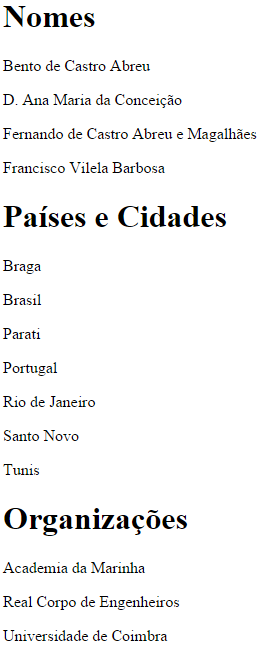
\includegraphics[scale=0.84]{html.png}

\subsection*{Exemplo 2}

\textbf{Texto de entrada:}

\begin{alltt}
<ENAMEX TYPE="PERSON">Luís Vaz de Camões</ENAMEX> 
(<ENAMEX TYPE="LOCATION">Lisboa</ENAMEX>,1524, 10 de Junho de 1580) 
foi um poeta de <ENAMEX TYPE="LOCATION">Portugal</ENAMEX>, 
considerado uma das maiores figuras da literatura em língua 
portuguesa e um dos grandes poetas do Ocidente. Pouco se sabe 
com certeza sobre a sua vida. Aparentemente nasceu em 
<ENAMEX TYPE="LOCATION" SUBTYPE="CITY">Lisboa</ENAMEX>, 
de uma família da pequena nobreza. Sobre a sua infância 
tudo é conjetura mas, ainda jovem, terá recebido uma sólida educação 
nos moldes clássicos, dominando o latim e conhecendo a literatura e a 
história antigas e modernas. Pode ter estudado na 
<ENAMEX TYPE="ORGANIZATION">Universidade de Coimbra</ENAMEX>,
mas a sua passagem pela escola não é documentada. Frequentou a corte de 
<ENAMEX TYPE="PERSON">D. João III</ENAMEX>, iniciou a sua carreira como 
poeta lírico e envolveu-se, como narra a tradição, em amores com damas 
da nobreza e possivelmente plebeias, além de levar uma vida boémia e  
turbulenta. Diz-se que, por conta de um amor frustrado, se autoexilou em 
<ENAMEX TYPE="LOCATION">África</ENAMEX>,alistado como militar, 
onde perdeu um olho em batalha. Voltando a 
<ENAMEX TYPE="LOCATION" SUBTYPE="COUNTRY">Portugal</ENAMEX>, feriu um servo 
do Paço e foi preso. Perdoado, partiu para o Oriente. Passando lá vários anos, 
enfrentou uma série de adversidades, foi preso várias vezes, combateu ao lado 
das forças portuguesas e escreveu a sua obra mais conhecida, a epopeia 
nacionalista Os Lusíadas. De volta à pátria, publicou Os Lusíadas e recebeu 
uma pequena pensão do rei <ENAMEX TYPE="PERSON">D. Sebastião</ENAMEX>
pelos serviços prestados à Coroa, mas nos seus anos finais parece 
ter enfrentado dificuldades para se manter.
\end{alltt}

\textbf{Comando utilizado:}

\begin{alltt}
./enamex < teste2 > teste2.html
\end{alltt}
\newpage
\textbf{Resultado (teste2.html), mostrado pelo browser:}

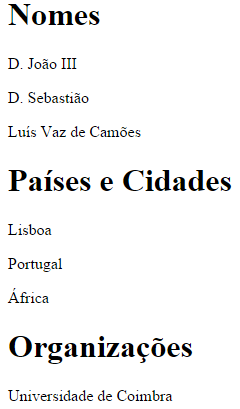
\includegraphics[scale=0.84]{html2.png}

\section{Conclusão}

Neste exercício do primeiro trabalho prático da disciplina de Processamento de Linguagens elaboramos um filtro que permite extrair de qualquer texto em notação Enamex os nomes, as localidades (quer sejam cidades ou países) e as organizações. Concutimos que usando o flex se poupa muitas linhas de código de outra linguagem, caso o filtro tivesse sido contruído integralmente em C, por exemplo. E é uma ferramenta simples, fácil de usar e cumpre a sua função. O filtro desenvolvido funciona e cumpre todos os requisitos do exercício, como era suposto. Foi desenvolvido em pouco tempo e foi testado várias vezes, até estar a cumprir o seu dever.


\end{document}
